\chapter{Partial-Derivative-Based Parser}
\label{sec:partial-derivative-parser}

Chapter~\ref{sec:derivative-parser} developed two parsers based on
Brzozowski's derivative. This chapter develops the corresponding two parsers
using Antimirov's partial derivative from
Section~\ref{sec:antimirov-partial-derivatives} in place of
$r\backslash x$ throughout.

The replacement is local in notation but affects how the parsers are constructed.
Both operators
consume one character and return the residual expression that remains to be
matched, and each operator is sufficient to drive a parser. However,
$r\backslash x$ returns a single expression, whereas $pd(r,x)$ returns a
\emph{set}, and a set has no single top-level alternation whose left branch a
rule can prefer. The POSIX choice performed by the two constructions of
Chapter~\ref{sec:derivative-parser}, in $\mathit{mkEps}$ and in
$\mathit{mkEpsBC}$, therefore has no corresponding site in the set
representation. The choice is relocated, and its outcome differs.

Section~\ref{sec:partial-derivative-parser-theory} identifies the new site,
and Sections~\ref{sec:pderiv-std-worked} and
\ref{sec:pderiv-bc-worked} demonstrate the consequence on a small
expression whose behaviour can be verified by direct inspection.

%
%
%

\section{The Frontier Approach}
\label{sec:partial-derivative-parser-theory}

Section~\ref{sec:antimirov-partial-derivatives} defined $pd(r,x)$ as a set
of residual expressions, each representing a state of the implicit NFA for
$r$ after reading $x$. Parsing therefore pairs each surviving element with
payload sufficient to reconstruct its parse tree: an injection closure in
this project's extension (Section~\ref{sec:pderiv-std-theory-rust}) or a bit
string in the reference-based construction
(Section~\ref{sec:pderiv-bc-theory}).

The algorithm maintains a \emph{frontier} of
\texttt{(residual, extra)} pairs, one per live \emph{strand}, and replaces
it after each input character with the successors produced by $pd$. At
end of input, it selects the first strand with a nullable residual.
Figure~\ref{fig:frontier} illustrates this process using
\texttt{pderiv\_bc}'s bits as payload; Section~\ref{sec:pderiv-std-theory-rust}
shows the frontier with injection closures.

Both strands in the last column are nullable, yet only the first is
inspected. Neither construction defines a preference; list order determines
which is considered first. This is deliberate: parse trees are complete only
at end of input and cannot be compared during pruning.
Sections~\ref{sec:pderiv-std-theory-rust} and
\ref{sec:pderiv-bc-theory} develop complete parsers from this loop.

\begin{figure}[ht]
\centering
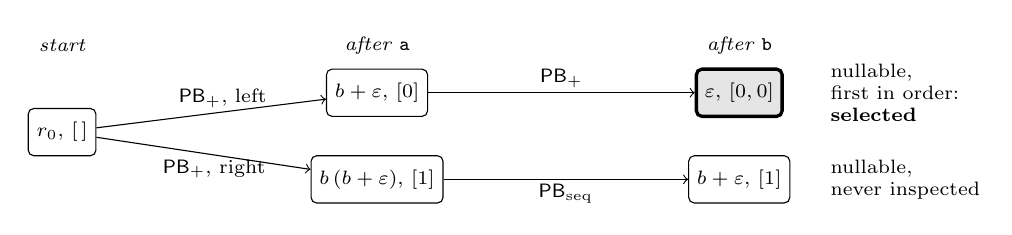
\begin{tikzpicture}[
  st/.style={draw, rounded corners=2pt, font=\scriptsize,
             minimum height=6mm, inner xsep=3pt},
  win/.style={st, fill=black!10, very thick},
  lbl/.style={font=\scriptsize, inner sep=1.5pt},
  col/.style={font=\scriptsize\itshape},
]
\node[col] (c0) at (0,2.1) {start};
\node[col] (c1) at (4.0,2.1) {after $\mathtt{a}$};
\node[col] (c2) at (8.6,2.1) {after $\mathtt{b}$};

\node[st] (s0) at (0,1.0) {$r_0$,\ $[\,]$};

\node[st] (a0) at (4.0,1.5) {$b+\varepsilon$,\ $[0]$};
\node[st] (a1) at (4.0,0.4) {$b\,(b+\varepsilon)$,\ $[1]$};

\node[win] (b0) at (8.6,1.5) {$\varepsilon$,\ $[0,0]$};
\node[st]  (b1) at (8.6,0.4) {$b+\varepsilon$,\ $[1]$};

\draw[->] (s0) -- node[lbl, above, pos=0.55] {$\mathsf{PB}_{+}$, left} (a0);
\draw[->] (s0) -- node[lbl, below, pos=0.55] {$\mathsf{PB}_{+}$, right} (a1);
\draw[->] (a0) -- node[lbl, above] {$\mathsf{PB}_{+}$} (b0);
\draw[->] (a1) -- node[lbl, below] {$\mathsf{PB}_{\mathrm{seq}}$} (b1);

\node[lbl, anchor=west, align=left] at (9.7,1.5)
  {nullable,\\first in order:\\\textbf{selected}};
\node[lbl, anchor=west, align=left] at (9.7,0.4)
  {nullable,\\never inspected};
\end{tikzpicture}
\caption{Frontier for $r_0 = (a+ab)(b+\varepsilon)$ on
\texttt{"ab"}, using \texttt{pderiv\_bc}'s bits as per-strand payload.
Both final strands are nullable; the first in list order is selected.}
\label{fig:frontier}
\end{figure}



%
%
%

\section{The Standard Partial-Derivative-Based Parser}
\label{sec:pderiv-std-theory-rust}

%
%
%

\section{The Bit-Coded Approach}
\label{sec:pderiv-bc-overview}

\texttt{pderiv\_std}'s frontier carries a chain of heap-allocated
closures, one per surviving derivative step, applied only once, on the
winning strand, at the very end. \texttt{pderiv\_bc} replaces that chain
with the same flat \texttt{Vec<bool>} Chapter~\ref{sec:derivative-parser}'s
\texttt{deriv\_bc} used, following Sulzmann's teaching-page Haskell
transcript \citep{sulzmann_slides} directly rather than building a
parallel construction from scratch. Figure~\ref{fig:frontier}
(Section~\ref{sec:partial-derivative-parser-theory}) already draws this
representation in full, so there is no second frontier diagram to
redraw here: reading it again now, the payload on every strand is a
\texttt{Vec<bool>}, not an $\iota$.

\paragraph{Comparison with the standard construction.}

\begin{center}
\begin{tabular}{@{}l>{\raggedright\arraybackslash}p{4.0cm}%
                  >{\raggedright\arraybackslash}p{4.0cm}@{}}
\hline
& \texttt{pderiv\_std} & \texttt{pderiv\_bc} \\
\hline
Per-strand payload & \texttt{Rc<dyn Fn>} closure chain & \texttt{Vec<bool>} \\
Allocation per step & one heap closure per successor & one \texttt{Vec} append \\
Residual constructor & plain \texttt{Regex::seq} only & \texttt{smart\_seq} where safe \\
Followed reference & none; this thesis's own & \texttt{pDerivBC} directly \\
\hline
\end{tabular}
\end{center}

Both constructions deduplicate identically, \texttt{nub\_tree} and
\texttt{nub2} apply the same keep-the-first rule to the same residual
equality, so the difference in this table is entirely about what rides
alongside the residual, never about which residual survives. The next
section develops \texttt{pderiv\_bc}'s rules formally and sets its own
per-case table next to Section~\ref{sec:pderiv-tree-theory}'s, now that
both constructions are available to compare.

%
%
%

\section{The Bit-Coded Partial-Derivative-Based Parser}
\label{sec:pderiv-bc-theory}

Sulzmann's teaching-page Haskell transcript gives a bit-coded
partial-derivative construction, \texttt{pDerivBC}, that this thesis's
\texttt{pderiv\_bc} follows directly \citep{sulzmann_slides}. It extends
$pd$ with per-strand bits the same way
Section~\ref{sec:bitcoded-optimization-theory}'s $\backslash_b$ extends
the Brzozowski derivative, with one visible difference: the bits stay
\emph{external} to the expression tree, as a plain list carried
alongside a plain, un-annotated $r$, instead of being folded into an
\texttt{ARegex}-shaped tree. This construction's correctness criterion is
literal agreement with \texttt{pDerivBC}, not an independently derived
ideal form.

\subsection{The Bit-Coded Partial Derivative}
\label{sec:pderivbc-rules-theory}

Writing $D_r$ for $\mathit{pDerivBC}(x,r)$ throughout, to keep the set
comprehensions readable, the base and non-sequence cases are

\begin{equation}\label{eq:pderivbc}
\begin{aligned}
D_{\varepsilon} &= \{\} \qquad\qquad D_{\emptyset} = \{\}
  &&(\mathsf{PB}_{\varepsilon}),\ (\mathsf{PB}_{\emptyset}) \\
D_{y} &= \begin{cases} \{(\varepsilon, [\,])\} & x = y \\
                       \{\} & x \neq y \end{cases}
  &&(\mathsf{PB}_{\mathrm{lit}}) \\
D_{r+s} &= \mathit{nub2}\big(
  \{(r', 0{:}bs) \mid (r',bs) \in D_r\} \\
  &\qquad\quad \cup\ \{(s', 1{:}bs) \mid (s',bs) \in D_s\}\big)
  &&(\mathsf{PB}_{+}) \\
D_{r^{*}} &= \mathit{nub2}\big(
  \{(\mathit{smartC}(r', r^{*}),\, 0{:}bs) \mid (r',bs) \in D_r\}\big)
  &&(\mathsf{PB}_{*})
\end{aligned}
\end{equation}

and the sequence case splits on the nullability of the left factor
exactly as Equation~\eqref{eq:derivative} does:

\begin{equation}\label{eq:pderivbc-seq}
\begin{aligned}
D_{rs} &= \{(\mathit{smartC}(r',s),\, bs) \mid (r',bs) \in D_r\}
  && (\mathsf{PB}_{\mathrm{seq}}),\ n(r) = \mathrm{false} \\
D_{rs} &= \mathit{nub2}\big(
  \{(r's,\ bs) \mid (r',bs) \in D_r\} \\
  &\qquad\quad \cup\ \{(s',\ \mathit{mkEpsBC}_r \mathbin{+\!\!+} bs)
       \mid (s',bs) \in D_s\}\big)
  && (\mathsf{PB}_{\mathrm{seq}}^{\,n}),\ n(r) = \mathrm{true}
\end{aligned}
\end{equation}

The names extend Section~\ref{sec:antimirov-partial-derivatives}'s
$\mathsf{P}$ scheme, one $\mathsf{PB}$ rule per $\mathsf{P}$ rule, and
the derivation below cites them with the binding of $r$ and $s$ given at
each application. Here $\mathit{mkEpsBC}_r$ is the plain-$r$ analogue of
Section~\ref{sec:mk-eps-bc}'s $\mathit{mkEpsBC}$, identical in structure
but walking an un-annotated tree; $\mathit{smartC}$ is the smart
concatenation constructor of
Section~\ref{sec:antimirov-partial-derivatives}, collapsing
$\varepsilon\cdot s$ to $s$; and \texttt{nub2} deduplicates a list of
\texttt{(residual, bits)} pairs by comparing the residual alone, keeping
the first occurrence.

Two details of Equation~\eqref{eq:pderivbc-seq} deserve attention.
$\mathsf{PB}_{\mathrm{seq}}^{\,n}$'s second set is where a strand
inherits $\mathit{mkEpsBC}_r$, the bits $r$ would have contributed by
matching empty, which is the same move
$\mathsf{B}_{\mathrm{seq}}^{\,n}$ made with $\mathit{fuse}$ in
Chapter~\ref{sec:derivative-parser} and the same one
$\mathsf{I}_{\mathrm{seq}}^{R}$ made with $\mathit{mkEps}$. And the two
sequence cases build their residuals differently:
$\mathsf{PB}_{\mathrm{seq}}$ uses $\mathit{smartC}$ while
$\mathsf{PB}_{\mathrm{seq}}^{\,n}$ builds its first strand with a plain
$r's$. That asymmetry is present in the reference itself and is
preserved here and not "corrected", since correctness of this
construction is judged by literal agreement with that reference
(Chapter~\ref{sec:evaluation}) and not against an independently derived
ideal form. Section~\ref{sec:pderiv-tree-theory} met the same question
from the other side, where the choice between the two constructors was
not free.

\paragraph{In Rust.}
\label{sec:pderiv-bc-theory-rust}

\texttt{pderiv\_bc} transcribes
$\mathit{pDerivBC}$ case for case. Each $D_r$ becomes a vector of
\texttt{(Regex, Vec<bool>)} pairs and not a set, because order is what
encodes priority here, and a \texttt{HashSet} would discard exactly the
information selection depends on. Deduplication is factored into its
own function, Figure~\ref{fig:nub2-rust}, used by every case that can
produce more than one strand.

\begin{figure}[H]
\begin{verbatim}
fn nub2(pairs: Vec<(Regex, Vec<bool>)>) -> Vec<(Regex, Vec<bool>)> {
    let mut seen: HashSet<Regex> = HashSet::with_capacity(pairs.len());
    let mut out = Vec::with_capacity(pairs.len());
    for (r, bs) in pairs {
        if seen.insert(r.clone()) {
            out.push((r, bs));
        }
    }
    out
}
\end{verbatim}
\caption{\texttt{nub2}: stable deduplication on the residual alone.
\texttt{HashSet::insert} returns \texttt{true} the first time a value is
seen and \texttt{false} on every repeat, so the loop keeps a pair
exactly when its residual has not been seen before, in the order the
input \texttt{Vec} presents them.}
\label{fig:nub2-rust}
\end{figure}

This is the one place in the codebase where \texttt{Regex}'s derived
\texttt{Hash} implementation (Section~\ref{sec:regex-rust-implementation})
is load-bearing: elsewhere equality alone would do, but a hash set is
what keeps \texttt{nub2} linear in the number of strands instead of
quadratic.

Figure~\ref{fig:pderivbc-rust} gives the two arms that produce more than
one strand and tag them as they go; \texttt{Star} is left out, since it
tags its one strand with a single leading \texttt{false} the same way
\texttt{Alt}'s left arm does, and otherwise matches
Figure~\ref{fig:derivbc-rust}'s star arm in Chapter~\ref{sec:derivative-parser}.

\begin{figure}[H]
\small
\begin{verbatim}
Regex::Alt(r1, r2) => {
    let mut out: Vec<(Regex, Vec<bool>)> = pderiv_bc(r1, x)
        .into_iter()
        .map(|(r1_, mut bs)| {
            let mut b = vec![false];
            b.append(&mut bs);
            (r1_, b)
        })
        .collect();
    out.extend(pderiv_bc(r2, x).into_iter().map(|(r2_, mut bs)| {
        let mut b = vec![true];
        b.append(&mut bs);
        (r2_, b)
    }));
    nub2(out)
}

Regex::Seq(r1, r2) => {
    if nullable(r1) {
        let mut out: Vec<(Regex, Vec<bool>)> = pderiv_bc(r1, x)
            .into_iter()
            .map(|(r1_, bs)| (Regex::seq(r1_, *r2.clone()), bs))
            .collect();
        let eps_bits = mk_eps_bits(r1);
        out.extend(pderiv_bc(r2, x).into_iter().map(|(r2_, bs)| {
            let mut b = eps_bits.clone();
            b.extend(bs);
            (r2_, b)
        }));
        nub2(out)
    } else {
        pderiv_bc(r1, x)
            .into_iter()
            .map(|(r1_, bs)| (smart_seq(r1_, r2), bs))
            .collect()
    }
}
\end{verbatim}
\caption{The alternation and sequence arms of \texttt{pderiv\_bc},
transcribing $\mathsf{PB}_{+}$, $\mathsf{PB}_{\mathrm{seq}}$ and
$\mathsf{PB}_{\mathrm{seq}}^{\,n}$.}
\label{fig:pderivbc-rust}
\end{figure}

\texttt{Alt} prepends its tag with \texttt{vec![false]}/\texttt{vec![true]}
and \texttt{append}, which is $0{:}bs$ and $1{:}bs$ read as a
\texttt{Vec} operation, then deduplicates the combined vector once at the
end, matching $\mathit{nub2}$'s position on the outside of the union in
Equation~\eqref{eq:pderivbc}.

\texttt{Seq} is the one place the two constructors genuinely differ, and
the code keeps that difference instead of smoothing it away. The
nullable branch's first strand is built with plain
\texttt{Regex::seq(r1\_, *r2.clone())}, matching
$\mathsf{PB}_{\mathrm{seq}}^{\,n}$'s plain $r's$; its second strand
reuses \texttt{mk\_eps\_bits(r1)} exactly as
Section~\ref{sec:pderivbc-rules-theory} described. The non-nullable branch,
reached only when \texttt{nullable(r1)} is false, calls
\texttt{smart\_seq(r1\_, r2)} instead, matching
$\mathsf{PB}_{\mathrm{seq}}$. A reader who only skims the two branches
could mistake this for an inconsistency; it is the literal transcription
of the asymmetry Equation~\eqref{eq:pderivbc-seq} already has.

\subsection{Comparing the Two Constructions}
\label{sec:pderiv-bc-comparison}

Section~\ref{sec:pderiv-tree-theory}'s table and this section's rules
are the same case split read twice, once attaching a closure and once a
bit:

\begin{center}
\begin{tabular}{lll}
\hline
Case & \texttt{pderiv\_bc} attaches & \texttt{pderiv\_tree} attaches \\
\hline
$\varepsilon$, $\emptyset$ & no strands & no strands \\
$x$ (matching) & \texttt{[]} & \texttt{|\_| Char(x)} \\
$r+s$, left & \texttt{0:}\textit{bs} & \texttt{|v| Left(inj1(v))} \\
$r+s$, right & \texttt{1:}\textit{bs} & \texttt{|v| Right(inj2(v))} \\
$rs$, continue $r$ & \textit{bs} & \texttt{|Pair(v1,v2)| Pair(inj1(v1), v2)} \\
$rs$, jump to $s$ & $\mathit{mkEpsBC}_r$ \texttt{++} \textit{bs} & \texttt{|v2| Pair(mk\_eps(r), inj2(v2))} \\
$r^{*}$ & \texttt{0:}\textit{bs} & \texttt{|Pair(v1,vs)| Star(inj1(v1) : vs)} \\
\hline
\end{tabular}
\end{center}

Every row is the same decision, expressed once as a bit and once as a
constructor. The correspondence is exact enough that the "jump to $s$"
row calls the shared \texttt{mk\_eps} at precisely the point
\texttt{pderiv\_bc} calls \texttt{mk\_eps\_bits}, for the reason
$\mathsf{I}_{\mathrm{seq}}^{R}$ gave in Chapter~\ref{sec:derivative-parser}.
\texttt{nub\_tree} is called in exactly the positions \texttt{nub2} is
in Figure~\ref{fig:pderivbc-rust}, deduplicating on the residual alone
and keeping the first occurrence, so the priority order is preserved
identically between the two constructions.

\paragraph{Where \texttt{nub2} is and is not applied.} \texttt{nub2}
appears inside $\mathit{pDerivBC}$, once per case that can produce more
than one strand, and nowhere else. In particular the frontier-driving
loop concatenates the per-strand results into the next frontier without
deduplicating across them, so the guarantee \texttt{nub2} provides is
local to a single strand's expansion and does not extend to the frontier
as a whole. Two strands that were distinct at step $i$ can converge on
the same residual at step $i+1$ and both survive, exactly the same
effect \texttt{nub\_tree} permits in \texttt{pderiv\_std}, since both
apply the same keep-the-first rule only within a single strand's
expansion.

\subsection{Parser}
\label{sec:pderiv-bc-driver}

\texttt{step\_frontier} and \texttt{select\_bits}
implement the loop of
Section~\ref{sec:partial-derivative-parser-theory}. Figure~\ref{fig:pderivbc-driver-rust}
gives both, plus the entry point that calls them.

\begin{figure}[H]
\begin{verbatim}
pub(super) fn step_frontier(frontier: &[(Regex, Vec<bool>)], x: char)
    -> Vec<(Regex, Vec<bool>)>
{
    let mut out = Vec::new();
    for (r, bits) in frontier {
        for (r_next, extra) in pderiv_bc(r, x) {
            let mut combined = bits.clone();
            combined.extend(extra);
            out.push((r_next, combined));
        }
    }
    out
}

pub(super) fn select_bits(frontier: &[(Regex, Vec<bool>)])
    -> Option<Vec<bool>>
{
    for (r, bits) in frontier {
        if nullable(r) {
            let mut result = bits.clone();
            result.extend(mk_eps_bits(r));
            return Some(result);
        }
    }
    None
}

pub fn parse_pderiv_bc(input: &str, r: &Regex) -> Option<ParseTree> {
    let mut frontier = vec![(r.clone(), Vec::new())];
    for c in input.chars() {
        frontier = step_frontier(&frontier, c);
        if frontier.is_empty() {
            return None;
        }
    }
    let bits = select_bits(&frontier)?;
    Some(decode(r, &bits))
}
\end{verbatim}
\caption{The frontier loop and its entry point. \texttt{step\_frontier}
replaces every \texttt{(residual, bits)} pair with the union of
\texttt{pderiv\_bc} applied to it, concatenating each result's bits onto
that strand's accumulated prefix. \texttt{select\_bits} scans in list
order and returns the first nullable strand's
\texttt{bits ++ mk\_eps\_bits(residual)}.}
\label{fig:pderivbc-driver-rust}
\end{figure}

\texttt{parse\_pderiv\_bc} drives the loop and passes the winning
bit-string, together with the \emph{original} \texttt{Regex} and never
the derived residual, to \texttt{decode} (Section~\ref{sec:decode}).
That is the same shared decoder \texttt{deriv\_bc} uses, since both
constructions arrive at the identical \texttt{(Regex, bits)} shape by
the time decoding is needed, whatever route each took to get there. The
early return on an empty frontier is the same short-circuit
Figure~\ref{fig:pderiv-loop-rust}'s matcher uses, now guarding a
\texttt{Vec<(Regex, Vec<bool>)>} instead of a \texttt{HashSet<Regex>}.

\subsection{Worked Example}
\label{sec:pderiv-bc-worked}

Run the same $r_0$ against $\mathtt{ab}$ through this construction,
checked against \texttt{cargo run -- parse "(a|ab)(b|)" "ab" --parser
pderiv\_bc --diag 3} (Appendix~\ref{app:report-pderiv-bc-match}), so it
can be read side by side with Section~\ref{sec:pderiv-std-worked}'s run
of the standard construction on the identical input.

\paragraph{Forward pass.}
The frontier starts as one strand, $(r_0,[\,])$. The first character
binds $r=a+ab$ and $s=b+\varepsilon$ at the outer node. That $r$ is not
nullable, so $\mathsf{PB}_{\mathrm{seq}}$ applies and $s$ contributes no
strand; the strands that do appear come from $\mathsf{PB}_{+}$
one level down:

\begin{equation}\label{eq:pd-step1}
\begin{aligned}
D_{a+ab}
&= \{(\varepsilon,[0])\} \cup \{(b,[1])\}
&&\mathsf{PB}_{+},\ r = a,\ s = ab \\
D_{r_0}
&= \{(\mathit{smartC}(\varepsilon,\, b+\varepsilon),\ [0]),\
    (\mathit{smartC}(b,\, b+\varepsilon),\ [1])\}
&&\mathsf{PB}_{\mathrm{seq}},\ n(a+ab) = \mathrm{false} \\
&= \{(b+\varepsilon,\ [0]),\ (b\,(b+\varepsilon),\ [1])\}
&&\mathsf{SC}\ \text{twice}
\end{aligned}
\end{equation}

The two applications of $\mathsf{SC}$ take different branches, which is
why the two strands look so different from
Section~\ref{sec:pderiv-std-worked}'s at the same step. Against the
first, $r' = \varepsilon$, so $\mathsf{SC}$ absorbs it and leaves
$b+\varepsilon$ alone; against the second, $r' = b \neq \varepsilon$, so
it keeps the concatenation. The trace agrees:

\begin{verbatim}
Step 1 (char: 'a', position 1)
      rule: pDerivBC('a', r1.r2)  [nullable(r1)=false]
           = [(smartC(r1',r2), bs) | (r1',bs) <- pDerivBC(c,r1)]
  frontier after (2 residual(s)):
    [0] Alt(Lit('b'), Eps)   bits = [0]
    [1] Seq(Lit('b'), Alt(Lit('b'), Eps))   bits = [1]
\end{verbatim}

Both bits were emitted by $\mathsf{PB}_{+}$ one level down, and
$\mathsf{PB}_{\mathrm{seq}}$ carried them outward unchanged, which is
why neither strand's bits grew at this step. Where the plain bit-coded
construction of Chapter~\ref{sec:derivative-parser} kept the two
alternatives inside one expression, joined by $\oplus$, they are now two
separate objects that will be advanced independently.

The second character steps \emph{both} strands, and each is matched
against the rule set on its own, so two different rules fire on the same
character:

\begin{equation}\label{eq:pd-step2}
\begin{aligned}
D_{b+\varepsilon}
&= \{(\varepsilon,[0])\} \cup \{\}
&&\mathsf{PB}_{+},\ r = b,\ s = \varepsilon;\ \mathsf{PB}_{\varepsilon} \\
D_{b\,(b+\varepsilon)}
&= \{(\mathit{smartC}(\varepsilon,\, b+\varepsilon),\ [\,])\}
   = \{(b+\varepsilon,\ [\,])\}
&&\mathsf{PB}_{\mathrm{seq}},\ n(b) = \mathrm{false}
\end{aligned}
\end{equation}

Strand \texttt{[0]} is an alternation whose left disjunct contributes
$\varepsilon$ tagged $0$ and whose right contributes nothing, since
$\mathsf{PB}_{\varepsilon}$ returns the empty set. Strand \texttt{[1]}
is a concatenation whose left factor is a bare literal, so
$\mathsf{PB}_{\mathrm{seq}}$ applies and only that factor is derived.
Each strand's accumulated bits are its own prefix followed by whatever
the step produced, so \texttt{[0]} gains a $0$ and reaches
\texttt{[0,0]} while \texttt{[1]} gains nothing and stays at
\texttt{[1]}:

\begin{verbatim}
Step 2 (char: 'b', position 2)
    from [0]:
      rule: pDerivBC('b', r1+r2) = tag(0, pDerivBC('b',r1)) ++
        tag(1, pDerivBC('b',r2)), nub2
      -> (Eps, [0])
    from [1]:
      rule: pDerivBC('b', r1.r2)  [nullable(r1)=false]
           = [(smartC(r1',r2), bs) | (r1',bs) <- pDerivBC(c,r1)]
      -> (Alt(Lit('b'), Eps), [])
  frontier after (2 residual(s)):
    [0] Eps   bits = [00]
    [1] Alt(Lit('b'), Eps)   bits = [1]
\end{verbatim}

\paragraph{Selection and result.}
Selection scans this final frontier in list order and takes the first
nullable strand. Strand \texttt{[0]}, $(\varepsilon,[0,0])$, is checked
and accepted before strand \texttt{[1]} is inspected, although
\texttt{[1]} is nullable too:

\begin{equation}\label{eq:pdbc-decode}
[0]\text{'s bits} \mathbin{+\!\!+} \mathit{mkEpsBC}(\varepsilon)
  = [0,0] \mathbin{+\!\!+} [\,] = [0,0],
\qquad
\mathit{decode}_{r_0}([0,0]) = \big(\mathit{Left}\ a,\ \mathit{Left}\ b\big).
\end{equation}

\begin{verbatim}
selected residual's accumulated bits ++ mkEpsBC(residual) = [00]

decode((a|ab)(b|), [00]):
  = (Left a, Left b)

RESULT
Bits:                 [00]
Parse tree:           (Left a, Left b)
Flattened:            "ab"
\end{verbatim}

This is the identical tree Section~\ref{sec:pderiv-std-worked} reached
by composing injection closures, reached here by reading bits off the
winning strand instead. Two differences from that section's trace are
visible, and both were predicted by the smart-constructor argument of
Section~\ref{sec:pderiv-tree-theory}. First, the residuals themselves:
where this construction lists \texttt{Alt(Lit('b'), Eps)} after
$\mathtt{a}$, Section~\ref{sec:pderiv-std-worked} lists
\texttt{Seq(Eps, Alt(Lit('b'), Eps))}, the $\varepsilon$ node
$\mathit{smartC}$ discards here and the other construction cannot
afford to. Second, and sharper: because the residuals differ, the two
constructions do not even take the same rules at step two. This
construction's strand \texttt{[0]} is an \texttt{Alt} and fires
$\mathsf{PB}_{+}$; the standard construction's is a \texttt{Seq} whose
left factor is the retained \texttt{Eps}, so it fires the nullable
sequence rule instead. The two constructions are therefore not running
over the same residuals, and not applying the same rules to them, and
they still select the same tree. Because deduplication runs on residual
syntax in both, they can in principle prune at different points as
well, which makes their agreement on every tested case a stronger check
than it would be if they shared a residual representation.

